\documentclass[11pt,a4paper]{article}
\usepackage[utf8]{inputenc}
\usepackage[T1]{fontenc}
\usepackage{lmodern}
\usepackage{textcomp}
\usepackage{amsmath,amssymb}
\usepackage{graphicx}
\usepackage{booktabs}
\usepackage{longtable}
\usepackage{array}
\usepackage{listings}
\usepackage{xcolor}
\usepackage[margin=1in]{geometry}
\usepackage{float}
\usepackage[hidelinks,breaklinks]{hyperref}
\usepackage{microtype}
\setlength{\parskip}{4pt}
\lstset{basicstyle=\ttfamily\scriptsize,breaklines=true,breakatwhitespace=false,
  postbreak=\mbox{\textcolor{gray}{$\hookrightarrow$}\space},frame=single,
  framerule=0.3pt,rulecolor=\color{gray!60},columns=fullflexible,keepspaces=true,
  showstringspaces=false,numbers=none,xleftmargin=4pt,xrightmargin=4pt,
  literate={\_}{{\_}}1}
\graphicspath{{figures/}}
\providecommand{\tightlist}{}
\title{Hydrostatic Mass Bias and Emulated Cluster Profile Evolution Between $z=0$ and $z=0.4987$}
\author{HEP-Genesis-Agent session record \\ \small Project: ramp-combo-cluster-profiles}
\date{2026-10-20}
\begin{document}
\maketitle
\noindent\textit{\small This document is an AI-generated account of an interactive session with the HEP-Genesis agent. Its text was written by a language model strictly from the session record; figures and numbers come only from tool results obtained during the session. The supplementary material and the transcript, generated alongside, document exactly what ran. Verify independently before use.}
\vspace{1em}

\begin{abstract}
We combine a literature survey of hydrostatic-equilibrium (HSE) mass bias in galaxy clusters with a test based on a HACC hydrodynamics emulator. The emulator returns gas-density (CGD), temperature (CTP) and pressure (CPP) profiles. The cluster-profile emulators are trained only up to $z=0.4987$, so the two redshifts compared are $z=0$ and $z=0.4987$. All seven emulator parameters were set to the midpoints of their design ranges.

From centred finite-difference log-slopes, the total slope at $R_{500c}$, $s_n+s_T$, is $-3.13\pm0.17$ at $z=0$ and $-3.24\pm0.17$ at $z=0.4987$. These agree within errors. The temperature at $R_{500}$ falls from $T/T_{500}=0.5916\pm0.0047$ to $0.5181\pm0.0101$.

Under an assumed $T_{500}$ convention we obtain $M_{\rm HSE}/M_{500}=0.925\pm0.051$ and $0.840\pm0.048$. In the FLAMINGO convention this is $b=-0.075$ and $-0.160$, a change $\Delta b=-0.085\pm0.070$ ($1.2\sigma$). The emulator's own pressure profile gives a consistent but equally insignificant change, $\Delta b=-0.066\pm0.055$. The sign agrees with the FLAMINGO cluster-scale trend. On this route, the change is driven by the temperature normalisation rather than by profile shape.

CPP agrees with CGD$\times$CTP at $R_{500}$ but is much shallower at $2R_{500}$, differing by 11--14$\sigma$. The three emulated profiles are therefore not mutually consistent at large radius. A non-thermal correction from the Nelson et al.\ fit over-corrects the emulator masses by 16--31\%; this result has low confidence and was contested.

Three parts of the study remain incomplete. A feedback-sensitivity run was produced but not reduced to numbers. The emulator exposes no halo mass, so a group-versus-cluster comparison was impossible. The absolute bias values depend on an undocumented temperature convention.
\end{abstract}

\section{Introduction}

The user asked for three things. The first was a survey of recent work on hydrostatic mass bias in galaxy clusters. The second was a set of predictions from a hydrodynamics emulator for the gas-density (CGD) and temperature (CTP) profiles at two redshifts. The third was a discussion of how evolution in profile shape affects hydrostatic mass reconstruction.

The session organised this request into six lines of work:
\begin{itemize}
\item emulator predictions, log-slopes and an HSE mass estimate at two redshifts;
\item a cited literature baseline;
\item robustness of the result to feedback and cosmology, plus the non-thermal fraction needed to remove the bias;
\item the mass dependence of the bias for groups versus clusters, added by the session's critic so the FLAMINGO result could be compared directly;
\item a significance test with a pressure-profile cross-check;
\item extraction of quantitative literature benchmarks from downloaded full texts.
\end{itemize}

The physical motivation is that the HSE mass at radius $r$ depends on the local temperature and on the logarithmic slopes $s_n=\mathrm{d}\ln n_{\rm gas}/\mathrm{d}\ln r$ and $s_T=\mathrm{d}\ln T/\mathrm{d}\ln r$. It does not depend on the density amplitude. Any redshift evolution of profile shape or temperature normalisation therefore feeds directly into the inferred bias.

The scope was limited by the emulator itself. Its cluster profiles exist only for $z\le0.4987$. It takes no halo-mass input. It does not document its $T_{500}$ definition or its temperature weighting.

\section{Methods}

\paragraph{Literature.}
Literature was collected with arXiv abstract searches, one web search, and metadata queries. Full texts were downloaded for four papers: arXiv:2409.07849 (FLAMINGO), arXiv:1805.00034 (X-COP), arXiv:1404.4636 (Nelson, Lau \& Nagai) and arXiv:2409.05815 (Simba). These were read in chunks. Verbatim quotes from all four were recorded in a bibliography file. The merger study arXiv:2511.10730 was used from its abstract only.

\paragraph{Emulator.}
The emulator was accessed through the \texttt{serve-hydro.sh} server, which lists 14 observables. The CGD, CTP and CPP profiles take redshift and seven parameters. Their ranges are:
\begin{itemize}
\item AGN wind coupling $\kappa_w\in[2,4]$;
\item AGN wind energy fraction $e_w\in[0.2,1.0]$;
\item black-hole seed mass $M_{\rm seed}/10^6\in[0.6,2.0]$;
\item kinetic feedback velocity $v_{\rm kin}/10^4\,\mathrm{km\,s^{-1}}\in[0.1,1.2]$;
\item kinetic feedback efficiency $\epsilon_{\rm kin}/10\in[0.02,1.2]$;
\item $\omega_m=\Omega_m h^2\in[0.12,0.155]$;
\item $\sigma_8\in[0.7,0.9]$.
\end{itemize}

No fiducial set is defined, so all parameters were placed at their range midpoints: $\kappa_w=3$, $e_w=0.6$, $M_{\rm seed}=1.3$, $v_{\rm kin}=0.65$, $\epsilon_{\rm kin}=0.61$, $\omega_m=0.1375$, $\sigma_8=0.8$.

Each prediction is a 19-bin logarithmic profile in $r/R_{500c}$ from 0.0154 to 2.74. Each bin carries a Gaussian-process mean and standard deviation. CGD is $\rho_{\rm gas}/\rho_{\rm crit}$, CTP is $T/T_{500}$, and CPP is $P/P_{500}$. CGD, CTP and CPP were predicted at $z=0$ and $z=0.4987$.

For the feedback test, CGD and CTP were also predicted at $\epsilon_{\rm kin}=0.02$ and $1.2$ at both redshifts, with the other parameters at their midpoints. Comparison overlays were produced with the server's plotting tool.

\paragraph{Slopes and masses.}
Log-slopes are centred finite differences in $\ln r$. The bin pairs used are (0.365, 0.649), (0.866, 1.155) and (1.540, 2.738) $R_{500c}$, which are labelled 0.49, 1.00 and 2.05 $R_{500c}$. Errors are propagated from the GP standard deviations, treating bins as independent. This was arithmetic performed by the assistant; no tool computes derivatives.

$T(R_{500})/T_{500}$ was taken as the geometric mean of the 0.866 and 1.155 bins. The assistant assumed $\mu=0.59$ and $kT_{500}=G\mu m_p M_{500}/(2R_{500})$, which gives
\begin{equation}
\frac{M_{\rm HSE}(R_{500})}{M_{500}} = -\frac{1}{2}\,\frac{T(R_{500})}{T_{500}}\,s,
\end{equation}
with $s=s_n+s_T$, or alternatively $s=s_P$ from CPP. The bias is quoted in the FLAMINGO convention, $b=(M_{\rm HSE}-M_{500})/M_{500}$. The $T_{500}$ convention is an assumption and is not documented by the emulator.

The Nelson et al.\ non-thermal fit was evaluated by hand at assumed values of $R_{500c}/R_{200m}$. Execution was local. The supplement holds the full tool-call log.

\section{Results}

\subsection{Literature baseline}

\paragraph{FLAMINGO (arXiv:2409.07849).}
This study defines $b_{\rm HSE}\equiv(M_{\rm HSE,500c}-M_{500c})/M_{500c}$. Its fiducial median bias goes from $\approx-0.1$ for groups to $\approx-0.2$ for clusters. The bias is nearly independent of the hydrostatic mass. The scatter at fixed true mass is smallest, $\sigma(b)\approx0.1$, at $M_{500c}\sim10^{14}\,M_\odot$.

At fixed true mass, hydrostatic masses increase with redshift on group scales and decrease with redshift on cluster scales, and the scatter grows. Models with lower gas fractions give more-biased group masses and less-biased cluster masses. The bias is insensitive to the analytic fitting function but sensitive to goodness of fit, with poorer fits giving stronger bias. The scatter comes from differences in pressure gradients rather than in temperature.

Further details were read from the full text but were contested by the critic, so we report them as such:
\begin{itemize}
\item all five profile methods converge to $b\approx-0.1$ for $10^{13.75}<M_{500c}<10^{14.25}\,M_\odot$;
\item the FLAMINGO calibration assumed a constant $b=-0.257$ from weak lensing;
\item volume-weighted profiles give a smaller, less mass-dependent bias than X-ray-weighted ones, with mass-weighted profiles in between, and the authors attribute most of the bias at $M_{500c}\gg10^{13}\,M_\odot$ to X-rays being a biased tracer;
\item $b(M)$ steepens with redshift over $z=0$--1.5 at fixed true mass, but is nearly unchanged at fixed $M_{\rm HSE}$ except at $z=1.5$.
\end{itemize}

\paragraph{X-COP (arXiv:1805.00034).}
For 13 nearby clusters, the median non-thermal pressure fraction is $\sim6\%$ at $R_{500}$ and $\sim10\%$ at $R_{200}$. This is lower than hydrodynamical simulations predict. With the Planck calibration the gas fractions imply $1-b=0.85\pm0.05$, with some evidence for a mass-dependent bias.

\paragraph{Nelson, Lau \& Nagai (arXiv:1404.4636).}
These authors used 65 simulated clusters with WMAP5 cosmology. They find that the non-thermal fraction profile is universal in redshift when radii are scaled to $R_{200m}$. It depends strongly on the mass accretion rate and is mostly radial. Their Eq.~7 is
\begin{equation}
\frac{P_{\rm rand}}{P_{\rm tot}} = 1 - A\left\{1+\exp\!\left[-\left(\frac{r/R_{200m}}{B}\right)^{\gamma}\right]\right\},
\end{equation}
with $A=0.452\pm0.001$, $B=0.841\pm0.008$ and $\gamma=1.628\pm0.019$. It is accurate to about 10\% over $0.1\le r/R_{200m}\le1.5$ out to $z=1.5$.

\paragraph{Simba (arXiv:2409.05815).}
Across six feedback variants, $10^{11}<M_{200c}<10^{14}\,M_\odot$ and $0<z<4$, gas-density profiles follow power laws. Their slope and amplitude depend only weakly on redshift at fixed mass. AGN jets make the profiles shallower above $M_{200c}\sim10^{13}\,M_\odot$.

\paragraph{Mergers (arXiv:2511.10730, abstract only).}
This AMR study finds that the bias dips sharply negative around a major merger, then shows a transient positive peak, then relaxes back. The behaviour is driven mainly by gas-density morphology and dynamics rather than thermodynamics.

\paragraph{Papers not read in detail.}
Several further papers were identified but not read: arXiv:1112.3659, arXiv:1308.6589, arXiv:1507.04338, arXiv:1608.04388, arXiv:1805.00035, arXiv:1805.00042, arXiv:2112.07554, arXiv:2010.00619, and arXiv:1306.3993 (named by the assistant without retrieved metadata).

\paragraph{Coverage of the baseline.}
Only four papers were cited with verbatim quotes, fewer than the session's own target of six. Early in the session the assistant also stated that none of its tools was a hydrodynamics emulator. That statement was wrong: the HACC emulator on \texttt{serve-hydro.sh} was subsequently used for all profile predictions.

\subsection{Emulated profiles at two redshifts}


\begin{figure}[H]
\centering
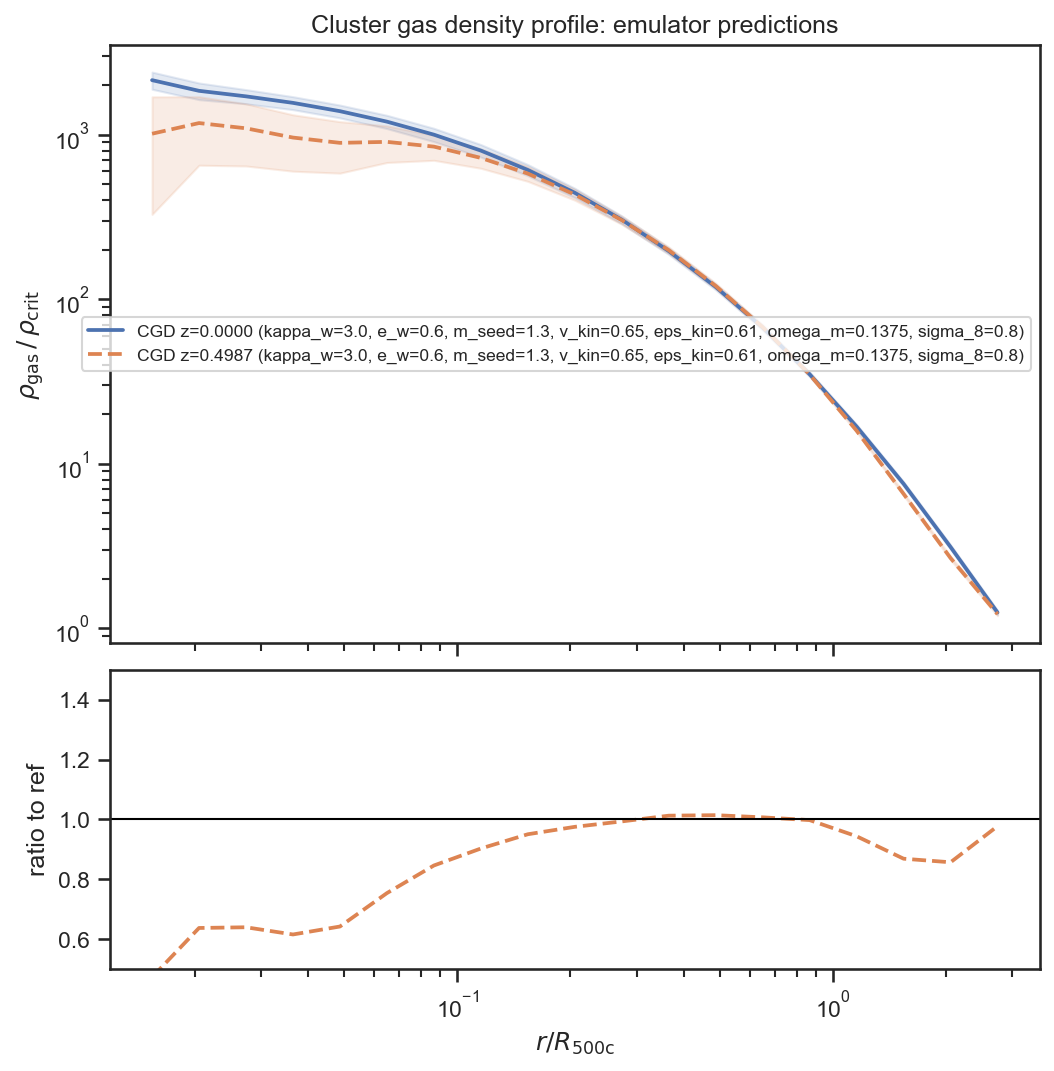
\includegraphics[width=0.85\textwidth,height=0.6\textheight,keepaspectratio]{fig-9.png}
\caption{CGD\_comparison.png Produced in this session by \texttt{plot\_observable\_comparison} on \textit{serve-hydro.sh}.}
\label{fig:9}
\end{figure}



Figure~\ref{fig:9} overlays CGD at $z=0$ and $z=0.4987$. Over 0.2--0.9 $R_{500c}$ the two redshifts agree within about 3\%. At $z=0.4987$ the density is about 6\% lower at $1.15R_{500c}$ and 13--14\% lower at 1.5--2.05 $R_{500c}$. It reconverges at $2.74R_{500c}$.

The core ($r<0.1R_{500c}$) appears 15--50\% lower at $z=0.4987$. The emulator uncertainty there is large, however: the innermost bin is $1018\pm689$ at $z=0.4987$ versus $2154\pm258$ at $z=0$. The core difference is therefore not significant.


\begin{figure}[H]
\centering
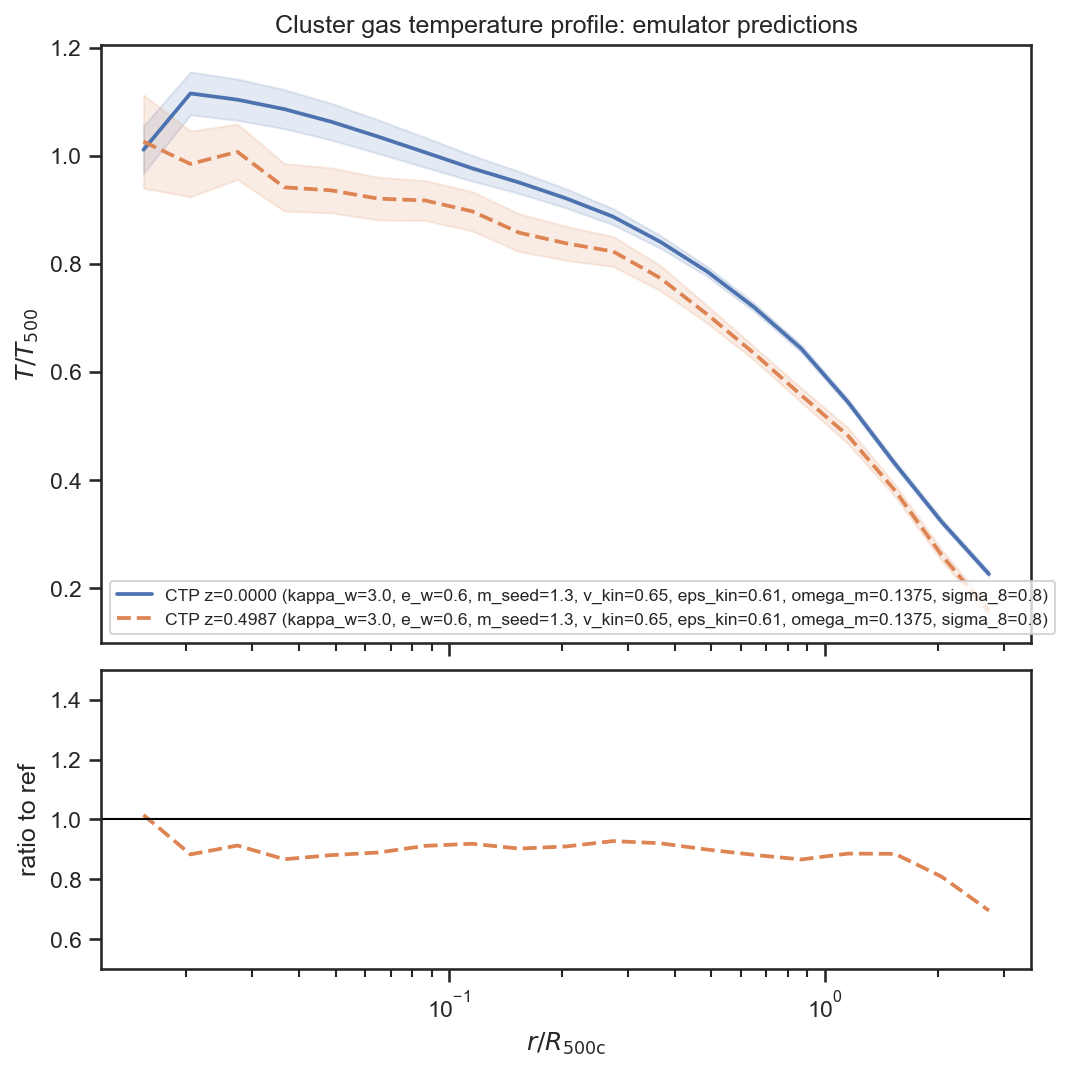
\includegraphics[width=0.85\textwidth,height=0.6\textheight,keepaspectratio]{fig-10.png}
\caption{CTP\_comparison.png Produced in this session by \texttt{plot\_observable\_comparison} on \textit{serve-hydro.sh}.}
\label{fig:10}
\end{figure}



Figure~\ref{fig:10} overlays CTP. Relative to $z=0$, $T/T_{500}$ at $z=0.4987$ is 7--13\% lower over 0.15--1.15 $R_{500c}$, 12\% lower at $R_{500c}$, and about 30\% lower at $2.74R_{500c}$. In scaled units, the dominant change between the redshifts is therefore in the temperature normalisation, not in the density profile.

\subsection{Log-slopes and the HSE mass ratio}

Table~\ref{tab:slopes} lists the slopes. The density slope does not evolve significantly at any of the three radii, in line with the Simba expectation. At $R_{500c}$ the slope sum is $-3.13\pm0.17$ at $z=0$ and $-3.24\pm0.17$ at $z=0.4987$.

The clearest change in shape is a steepening of $s_T$ at $2.05R_{500c}$, from $-1.12$ to $-1.54$, nominally about $3.6\sigma$. This rests on finite differences of emulator means with independent errors and was not checked against a smooth fit.

As a direct check on the arithmetic, the $z=0$ density slope near $R_{500c}$ is $\ln(16.862/35.076)/\ln(1.1548/0.8660)\approx-2.55$.

\begin{table}
\centering
\begin{tabular}{lcccc}
\toprule
$r/R_{500c}$ & $s_n$ ($z=0$) & $s_n$ ($z=0.4987$) & $s_T$ ($z=0$) & $s_T$ ($z=0.4987$)\\
\midrule
0.49 & $-1.86\pm0.10$ & $-1.87\pm0.10$ & $-0.27\pm0.03$ & $-0.35\pm0.06$\\
1.00 & $-2.55\pm0.16$ & $-2.74\pm0.10$ & $-0.58\pm0.06$ & $-0.50\pm0.14$\\
2.05 & $-3.13\pm0.07$ & $-2.93\pm0.06$ & $-1.12\pm0.05$ & $-1.54\pm0.11$\\
\bottomrule
\end{tabular}
\caption{Centred finite-difference log-slopes of the emulated profiles at midpoint parameters.}
\label{tab:slopes}
\end{table}

With $T(R_{500})/T_{500}=0.5916\pm0.0047$ ($z=0$) and $0.5181\pm0.0101$ ($z=0.4987$), the first estimate of the mass ratio was $M_{\rm HSE}/M_{500}=0.925$ and $0.840$. The ratio between the redshifts is 0.91.

The critic marked this finding as contested for two reasons. Its significance had not been tested, and its sign convention initially differed from FLAMINGO's. The follow-up below addresses both points.

\subsection{Pressure-profile cross-check and significance}

Table~\ref{tab:cpp} compares the CPP slope with $s_n+s_T$ over the same bin pairs. At $R_{500}$ the two routes agree within $0.4\sigma$. At $0.49R_{500}$ they differ by $1.3\sigma$ at $z=0$ and $2.4\sigma$ at $z=0.4987$. At $2.05R_{500}$ they disagree by $14\sigma$ and $11\sigma$. Beyond $R_{500}$, CPP is therefore not the product of CGD and CTP.

\begin{table}
\centering
\begin{tabular}{llccc}
\toprule
Radius & $z$ & $s_P$ (CPP) & $s_n+s_T$ & Difference\\
\midrule
$0.49R_{500}$ & 0 & $-1.981\pm0.042$ & $-2.133\pm0.104$ & $1.3\sigma$\\
$0.49R_{500}$ & 0.4987 & $-1.874\pm0.088$ & $-2.218\pm0.117$ & $2.4\sigma$\\
$1.00R_{500}$ & 0 & $-3.052\pm0.113$ & $-3.128\pm0.171$ & $0.37\sigma$\\
$1.00R_{500}$ & 0.4987 & $-3.232\pm0.154$ & $-3.243\pm0.172$ & $0.05\sigma$\\
$2.05R_{500}$ & 0 & $-2.877\pm0.042$ & $-4.249\pm0.086$ & $14.4\sigma$\\
$2.05R_{500}$ & 0.4987 & $-1.815\pm0.207$ & $-4.463\pm0.125$ & $10.9\sigma$\\
\bottomrule
\end{tabular}
\caption{Pressure-slope cross-check between CPP and CGD$\times$CTP.}
\label{tab:cpp}
\end{table}

Table~\ref{tab:mass} gives the mass ratios with the $T(R_{500})/T_{500}$ error propagated. The density-plus-temperature route gives $b=-0.075\pm0.051$ at $z=0$ and $b=-0.160\pm0.048$ at $z=0.4987$. The pressure route gives $b=-0.097\pm0.034$ and $b=-0.163\pm0.043$.

Both routes give a bias that becomes more negative with redshift. This is the same direction as FLAMINGO finds on cluster scales. Neither change is significant: each is $1.2\sigma$, and correlated emulator errors, which were not modelled, could move this significance in either direction. Because the slope sum at $R_{500}$ hardly changes, the larger nominal bias at $z=0.4987$ comes from the 12\% lower $T(R_{500})/T_{500}$, not from profile shape.

\begin{table}
\centering
\begin{tabular}{lccccc}
\toprule
Slope & $z=0$ & $z=0.4987$ & Difference & $\Delta b$ & Signif.\\
\midrule
$s_n+s_T$ & $0.925\pm0.051$ & $0.840\pm0.048$ & $0.085\pm0.070$ & $-0.085\pm0.070$ & $1.2\sigma$\\
$s_P$ (CPP) & $0.903\pm0.034$ & $0.837\pm0.043$ & $0.066\pm0.055$ & $-0.066\pm0.055$ & $1.2\sigma$\\
\bottomrule
\end{tabular}
\caption{$M_{\rm HSE}/M_{500}$ at $R_{500}$ and its redshift change, under the assumed $T_{500}$ convention.}
\label{tab:mass}
\end{table}

\subsection{Feedback sensitivity (not reduced)}

The assistant chose $\epsilon_{\rm kin}$ as the feedback lever. This was a judgement call, because the emulator does not indicate which parameter controls the profile slopes.


\begin{figure}[H]
\centering
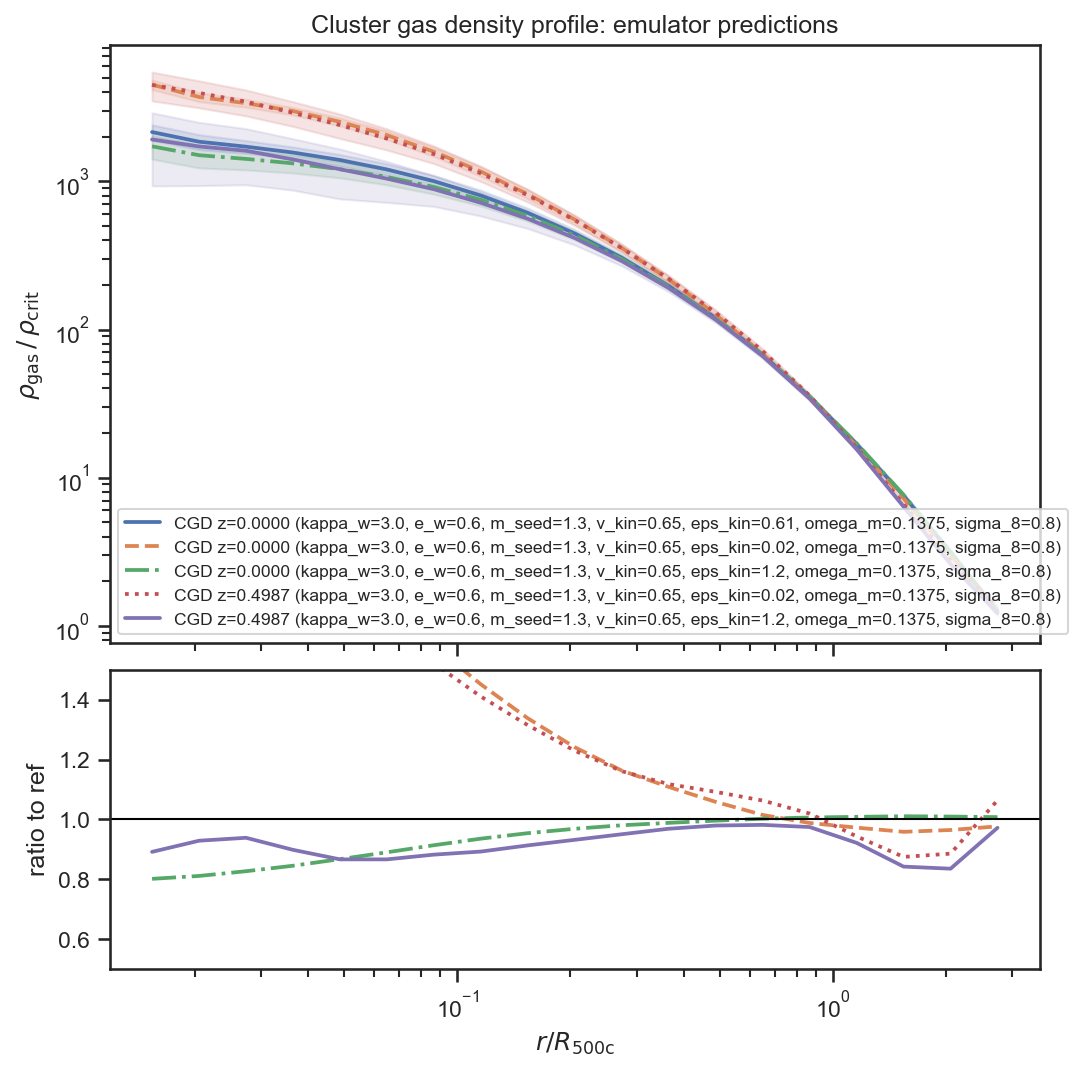
\includegraphics[width=0.85\textwidth,height=0.6\textheight,keepaspectratio]{fig-21.png}
\caption{CGD\_comparison.png Produced in this session by \texttt{plot\_observable\_comparison} on \textit{serve-hydro.sh}.}
\label{fig:21}
\end{figure}




\begin{figure}[H]
\centering
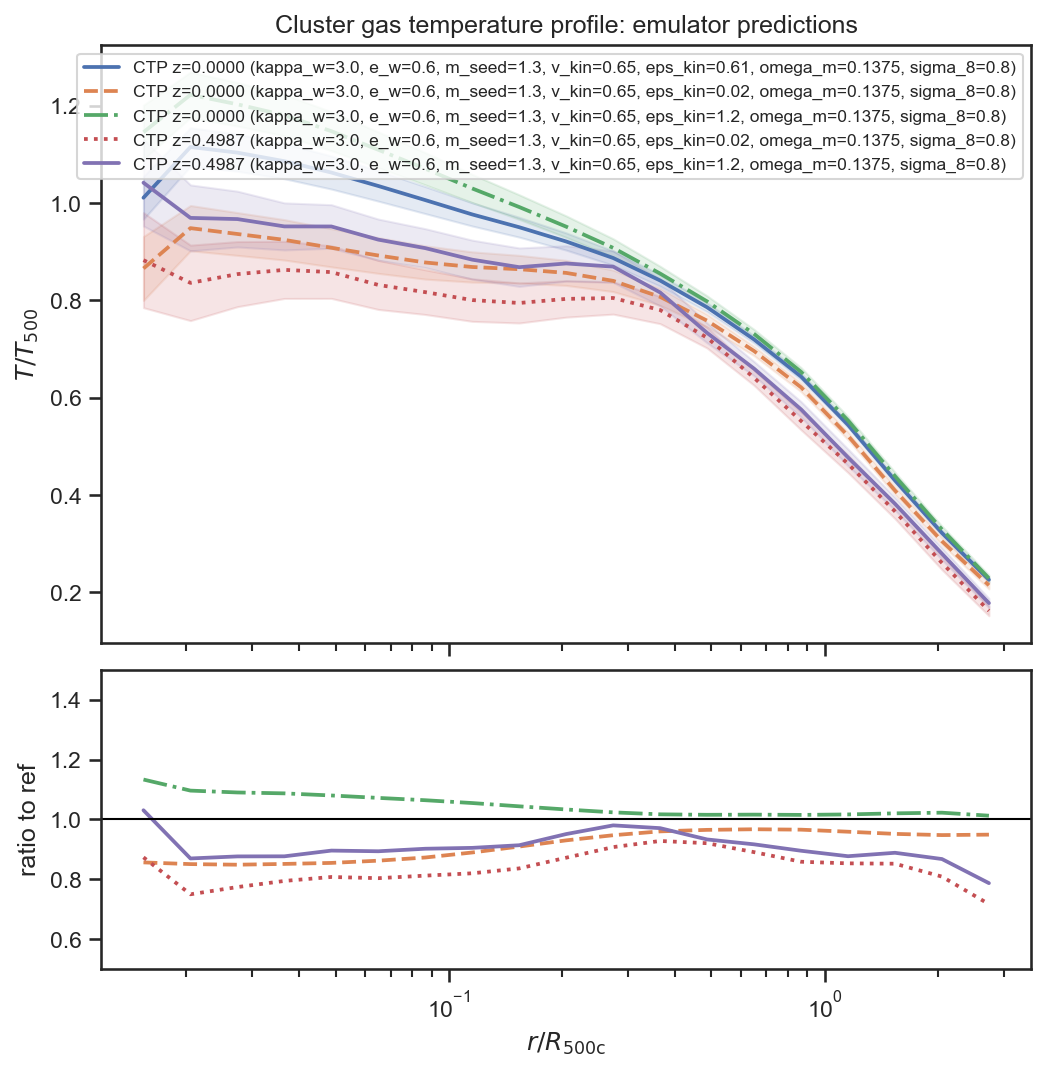
\includegraphics[width=0.85\textwidth,height=0.6\textheight,keepaspectratio]{fig-22.png}
\caption{CTP\_comparison.png Produced in this session by \texttt{plot\_observable\_comparison} on \textit{serve-hydro.sh}.}
\label{fig:22}
\end{figure}



Figure~\ref{fig:21} (CGD) and Figure~\ref{fig:22} (CTP) each overlay five profiles. These are the $z=0$ midpoint run ($\epsilon_{\rm kin}=0.61$) and the $\epsilon_{\rm kin}=0.02$ and $1.2$ runs at both redshifts.

The slopes, $T/T_{500}$ and $M_{\rm HSE}/M_{500}$ were not extracted from these runs. It therefore remains unknown whether feedback moves the bias more or less than the redshift change does. The fGas observable was not run, and no cosmological parameter was varied. This line of work is blocked or incomplete.

\subsection{Non-thermal correction}

The assistant assumed $R_{500c}\approx0.5$--$0.6\,R_{200m}$, nearer 0.5 at $z=0$ and 0.55--0.6 at $z=0.5$. Evaluating the Nelson et al.\ fit by hand at $x=r/R_{200m}=0.50$, 0.55 and 0.60 gives $f_{\rm nth}=0.254$, 0.274 and 0.294. The corresponding correction factors are $1/(1-f_{\rm nth})=1.34$, 1.38 and 1.42. This evaluation was contested by the critic.

Applying the factors to the emulator ratios gives 1.24--1.31 at $z=0$ and 1.16--1.19 at $z=0.4987$, an overcorrection of 16--31\%. Removing the bias in the emulator directly would require only $f_{\rm nth}\approx0.075$ ($z=0$) and $0.16$ ($z=0.4987$). These values are closer to the X-COP $\sim6\%$ at $R_{500}$.

The assistant proposed that the emulator's $T_{500}$ convention or temperature weighting may already absorb part of the bias. This finding carries low confidence and was contested. It depends entirely on the undocumented $T_{500}$ convention and on the hand-computed radius conversion.

\section{Discussion}

The emulator test gives a nuanced answer to how profile-shape evolution affects mass reconstruction. Between $z=0$ and $z=0.4987$ at midpoint parameters, the slope sum at $R_{500c}$ is unchanged within errors, and the density slope does not evolve. Together with the weak redshift dependence of density slopes reported by Simba (arXiv:2409.05815), this suggests that, at $R_{500}$, the density profile shape is not what drives bias evolution.

The nominal increase of the bias with redshift comes from the lower scaled temperature at $R_{500}$. Its direction matches the FLAMINGO cluster-scale trend (arXiv:2409.07849). It is, however, only a $1.2\sigma$ effect, and the absolute values depend on an assumed $T_{500}$ normalisation. The only shape change of nominal significance is the steepening of the temperature slope at $2R_{500c}$. Its consequence for masses at large radius is clouded by the inconsistency between CPP and CGD$\times$CTP there.

That inconsistency is a substantive limitation. At $2.05R_{500}$, $s_P=-2.88$ against $s_n+s_T=-4.25$ at $z=0$. The CPP profile could be a mean of per-halo products, a differently weighted quantity, or a different halo sample. The session did not establish which, or which profile is the appropriate input for hydrostatic masses beyond $R_{500}$.

The comparison with FLAMINGO's weighting results is also limited by the undocumented temperature weighting of CTP. FLAMINGO attributes much of the bias at cluster masses to X-ray weighting. Whether CTP is mass-weighted, emission-weighted or spectroscopic-like therefore matters directly.

Several planned items failed or were abandoned:
\begin{itemize}
\item The group-versus-cluster test is a dead end with this emulator: there is no mass input, no mass bins and no true $M_{500c}$, and redshift coverage stops at $z=0.4987$, so the FLAMINGO sign-flip between groups and clusters could not be tested.
\item The search for documentation of the HACC mass selection and temperature weighting was not run because the tool budget ran out.
\item The X-COP universal-profile slope comparison (arXiv:1805.00042) was not run, for the same reason.
\item The FLAMINGO quotes were not added to the bibliography.
\item A separate prediction plot with uncertainty bands was not produced.
\end{itemize}
Throughout, errors treat bins and redshifts as independent. The finite-difference slopes were not validated against smooth fits.

\section{Conclusions}

Four results were established. At design-midpoint parameters, the HACC emulator gives essentially unchanged log-slopes at $R_{500c}$ between $z=0$ and $z=0.4987$. It gives a 12\% lower scaled temperature at $R_{500}$ at the higher redshift. Under an assumed $T_{500}$ convention, it gives a bias of $b=-0.075\pm0.051$ to $-0.160\pm0.048$ (density plus temperature) or $-0.097\pm0.034$ to $-0.163\pm0.043$ (pressure). The redshift change is in the FLAMINGO cluster-scale direction but only $1.2\sigma$. Finally, CPP agrees with CGD$\times$CTP at $R_{500}$ and strongly disagrees at $2R_{500}$.

A literature baseline was assembled from FLAMINGO, X-COP, Nelson et al.\ and Simba, with the merger study used from its abstract. Some FLAMINGO full-text details and the non-thermal comparison remain contested. The latter carries low confidence.

Open items raised in the session:
\begin{enumerate}
\item extract $s_n+s_T$, $T/T_{500}$ and $M_{\rm HSE}/M_{500}$ from the $\epsilon_{\rm kin}=0.02$ and $1.2$ runs and compare the feedback-induced change with the redshift change;
\item determine the halo-mass selection behind the CGD/CTP/CPP profiles, the $T_{500}$ definition and the temperature weighting;
\item explain why CPP is much shallower than CGD$\times$CTP beyond $R_{500}$, and decide which profile to use for hydrostatic masses there;
\item complete the X-COP (arXiv:1805.00042) slope comparison and the remaining numerical extractions from FLAMINGO and Simba.
\end{enumerate}

\section*{References}
\begin{itemize}
\item arXiv:2409.07849 --- Hydrostatic mass bias for galaxy groups and clusters in the FLAMINGO simulations. J. Braspenning, J. Schaye, M. Schaller, R. Kugel, S. T. Kay (2024).
\item arXiv:1805.00034 --- Non-thermal pressure support in X-COP galaxy clusters. D. Eckert et al. (2018).
\item arXiv:1404.4636 --- Hydrodynamic Simulation of Non-thermal Pressure Profiles of Galaxy Clusters. K. Nelson, E. T. Lau, D. Nagai (2014).
\item arXiv:2409.05815 --- The impact of feedback on the evolution of gas density profiles from galaxies to clusters: a universal fitting formula from the Simba suite of simulations. D. Sorini, S. Bose, R. Davé, D. Anglés-Alcázar (2024).
\item arXiv:2511.10730 --- The signature of major mergers on the hydrostatic mass bias of galaxy clusters. I. Barranco-Llorca, D. Vallés-Pérez, S. Planelles, V. Quilis (2025).
\item arXiv:1112.3659 --- Evolution of the Merger Induced Hydrostatic Mass Bias in Galaxy Clusters.
\item arXiv:1308.6589 --- Weighing Galaxy Clusters with Gas. II. On the Origin of Hydrostatic Mass Bias in LambdaCDM Galaxy Clusters.
\item arXiv:1507.04338 --- Analytical model for non-thermal pressure in galaxy clusters - III. Removing the hydrostatic mass bias.
\item arXiv:1608.04388 --- Mass modeling of galaxy clusters: quantifying hydrostatic bias and contribution from non-thermal pressure.
\item arXiv:1805.00035 --- Hydrostatic mass profiles in X-COP galaxy clusters.
\item arXiv:1805.00042 --- Universal thermodynamic properties of the intracluster medium over two decades in radius in the X-COP sample.
\item arXiv:2112.07554 --- Tracing the non-thermal pressure and hydrostatic bias in galaxy clusters.
\item arXiv:2010.00619 --- The CAMELS project: Cosmology and Astrophysics with MachinE Learning Simulations.
\item arXiv:1306.3993 --- identifier named in the session; title not retrieved.
\end{itemize}

\section*{Data and code availability}
All outputs of this session are collected in the project folder \href{file:///Users/nramachandra/hep-genesis-testing/projects/ramp-combo-cluster-profiles}{\texttt{/\allowbreak{}Users/\allowbreak{}nramachandra/\allowbreak{}hep-genesis-testing/\allowbreak{}projects/\allowbreak{}ramp-combo-cluster-profiles}}.
The session produced 18 data files; the supplement lists them.
Full documentation of how these results were obtained is in the supplementary material (\texttt{supplement.pdf}: implementation details, the tool-call log, the research board with every finding and its evidence, figures not shown here, and the code index) and the verbatim transcript (\texttt{transcript.pdf}), generated alongside this report.


\end{document}
